\documentclass[11pt,twoside]{article}
\usepackage[T1]{fontenc}
\usepackage[utf8]{inputenc}
\usepackage[english]{babel}
\usepackage{amsmath}
\usepackage{amscd}
\usepackage{amssymb}
\usepackage{multirow}
\usepackage{tabularx}
\usepackage{graphicx}
\usepackage{url}
\usepackage{fancyhdr}
\usepackage{mathtools}
\usepackage{hyperref}
\usepackage{lastpage}
\usepackage[a4paper,margin=2.5cm,hmarginratio=1:1]{geometry}

%%%%%%%%%%%%%%%%%%%%%%%%%%%%%%%%%%%%%%%%%%%%%%%%%%%%%%%%%%%%%%%%%%%%%%%%%%%
%%%%%%%%%%%%%% ENTER YOUR PERSONAL INFORMATION HERE %%%%%%%%%%%%%%%%%%%%%%%
%%%%%%%%%%%%%%%%%%%%%%%%%%%%%%%%%%%%%%%%%%%%%%%%%%%%%%%%%%%%%%%%%%%%%%%%%%%


% Your name, personal number, and email.
\newcommand{\firstname}{Bastian}
\newcommand{\lastnames}{Fredriksson}
\newcommand{\persnr}{199302164216}
\newcommand{\email}{bastianf@kth.se}


% Your two study pals. Leave empty as necessary.
\newcommand{\studypalX}{Fabian Ström}
\newcommand{\studypalXemail}{fabstr@kth.se}
\newcommand{\studypalY}{}
\newcommand{\studypalYemail}{}


%%%%%%%%%%%%%%%%%%%%%%%%%%%%%%%%%%%%%%%%%%%%%%%%%%%%%%%%%%%%%%%%%%%%%%%%%%%
%%%%%%%%%%%%% DO NOT TOUCH ANYTHING BELOW THIS LINE %%%%%%%%%%%%%%%%%%%%%%%
%%%%%%%%%%%%%%%%%%%%%%%%%%%%%%%%%%%%%%%%%%%%%%%%%%%%%%%%%%%%%%%%%%%%%%%%%%%

\newcounter{problem}
\renewcommand\theproblem{\arabic{problem}}
\newenvironment{problem}{%
  \bigbreak
  \refstepcounter{problem}\noindent
  \llap{\textbf{\theproblem}\quad}\ignorespaces
}{%
  \par\if@nadaten@solutions\relax\else\filbreak\fi
}
\newenvironment{problem*}{%
  \bigbreak
  \refstepcounter{problem}\noindent
  \llap{\textbf{\theproblem}\quad}\ignorespaces
}{%
  \par
}
\newcounter{subproblem}[problem]
\renewcommand{\thesubproblem}{\arabic{problem}\alph{subproblem}}
\newenvironment{subproblem}{%
  \refstepcounter{subproblem}%
  \list{}{}%
  \item\leavevmode
  \llap{\hbox to \leftmargini{\textbf{\thesubproblem}\hfil}}%
  \ignorespaces
}{%
  \endlist\if@nadaten@solutions\relax\else\filbreak\fi
}
\newenvironment{subproblem*}{%
  \refstepcounter{subproblem}%
  \list{}{}%
  \item\leavevmode
  \llap{\hbox to \leftmargini{\textbf{\thesubproblem}\hfil}}%
  \ignorespaces
}{%
  \endlist
}

\newcommand{\homeworknr}{3}
\newcommand{\studentname}{\firstname~\lastnames}
\newcommand{\homework}{Homework~\homeworknr}
\newcommand{\coursenumber}{DD2448}
\newcommand{\coursename}{\coursenumber~Foundations of cryptography}
\newcommand{\coursenick}{krypto15}

\lhead[\studentname]{\coursename}
\chead{}
\rhead[\coursename]{\studentname}
\lfoot[\thepage~(\pageref{LastPage})]{}
\cfoot{}
\rfoot[]{\thepage~(\pageref{LastPage})}

\fancypagestyle{firststyle}
{
   \fancyhf{}
   \fancyfoot[R]{\thepage~(\pageref{LastPage})}
}

\renewcommand{\headrulewidth}{0pt}


%%%%%%%%%%%%%%%%%%%%%%%%%%%%%%%%%%%%%%%%%%%%%%%%%%%%%%%%%%%%%%%%%%%%%%%%%%%
%%% HERE YOU CAN ADD YOUR OWN MACROS AND ENVIRONMENTS IN THE PREAMBLE %%%%%
%%%%%%%%%%%%%%%%%%%%%%%%%%%%%%%%%%%%%%%%%%%%%%%%%%%%%%%%%%%%%%%%%%%%%%%%%%%

% Add your macros here.


\begin{document}

%%%%%%%%%%%%%%%%%%%%%%%%%%%%%%%%%%%%%%%%%%%%%%%%%%%%%%%%%%%%%%%%%%%%%%%%%%%
%%%%%%%%%%%% THE FOLLOWING GENERATES THE HEADER %%%%%%%%%%%%%%%%%%%%%%%%%%%
%%%%%%%%%%%% DO NOT TOUCH THIS %%%%%%%%%%%%%%%%%%%%%%%%%%%%%%%%%%%%%%%%%%%%
%%%%%%%%%%%%%%%%%%%%%%%%%%%%%%%%%%%%%%%%%%%%%%%%%%%%%%%%%%%%%%%%%%%%%%%%%%%

\thispagestyle{firststyle}

\noindent
\hspace{0.3cm}{\huge\textbf{\coursename}}

\noindent
\rule{\textwidth}{1pt}

\vspace{0.3cm}

\noindent
\begin{tabularx}{\textwidth}{lXl}
  \multirow{3}{*}{\textbf{\huge\homework}} && {\Large\textbf{\studentname}} \\
&&\\[-0.3cm]
  && {\Large\persnr} \\
&&\\[-0.35cm]
  && {\Large\texttt{\email}} \\
&&\\[-0.2cm]
\cline{3-3}
&&\\[-0.2cm]
  \multirow{2}{*}{\textbf{\huge\coursenick}} && {\small\studypalX, \texttt{\studypalXemail}} \\
&& {\small\studypalY \texttt{\studypalYemail}}
\end{tabularx}

\vspace{0.2cm}
\noindent
\rule{\textwidth}{1pt}

\vspace{0.5cm}

\pagestyle{fancy}

%%%%%%%%%%%%%%%%%%%%%%%%%%%%%%%%%%%%%%%%%%%%%%%%%%%%%%%%%%%%%%%%%%%%%%%%%%%
%%%%%%%%%%%%%%%%%%%%% YOUR SOLUTIONS START HERE %%%%%%%%%%%%%%%%%%%%%%%%%%%
%%%%%%%%%%%%%%%%%%%%%%%%%%%%%%%%%%%%%%%%%%%%%%%%%%%%%%%%%%%%%%%%%%%%%%%%%%%
%%                                                                       %%
%%  Do NOT remove any problem-, or subproblem environments below. If     %%
%%  you can not solve a problem, then you MUST simply leave the "NOT     %%
%%  SOLVED" string intact. This ensures that the numbering is correct    %%
%%  and it simplifies grading, leaving more time to prepare lectures     %%
%%  and help students.                                                   %%
%%                                                                       %%
%%  Do not remove any point markers. Leaving them in place simplifies    %%
%%  grading.                                                             %%
%%                                                                       %%
%%%%%%%%%%%%%%%%%%%%%%%%%%%%%%%%%%%%%%%%%%%%%%%%%%%%%%%%%%%%%%%%%%%%%%%%%%%

\begin{problem}
  (12I) IMPLEMENTED\\
  SHA-256 was implemented from the description available here:\\
  
  \url{https://helix.stormhub.org/papers/SHA-256.pdf}\\
  
  \noindent I also used the FIPS-specification during debugging. The RotR-operation was taken from Wikipedia: \\
  
  \url{http://en.wikipedia.org/wiki/Circular_shift}
\end{problem}

\begin{problem}
  (10I) IMPLEMENTED\\
  In this implementation, I've used the formulas on Wikipedia for calculating the tangent, finding the third point and calculating $Ge$ using double and add (I think the ModExp implementation would work too).\\
  
  \url{http://en.wikipedia.org/wiki/Elliptic_curve_point_multiplication}
\end{problem}

\begin{problem}
  \begin{subproblem}
    (8T)
In this problem I will assume that $H$ is a collision-resistant hash function. I will further assume that only one of the devices $R$ has access to the message which should be hashed (it would be possible to skip this assumption, i.e the message might reside on a shared network resource, and the overall scheme would still work). The purpose of the other machines in the network is to help $R$ to calculate the final hash as fast as possible without hogging the CPU of any machine in the network. 

The overall idea is to divide the blocks in a fair way between the computers, i.e a device with high computational power should be handed a larger amount of blocks than a computationally weak device. The devices are ordered in a tree-like fashion where each device has a parent and at most two children. The root $R$ of the tree is the computer who has the message to be hashed. The purpose of this computer is to distribute the blocks. Blocks processed by a child are sent to the parent. The parent computes the hash $h_{p}$ for the blocks it received from $R$ and waits for the children to send their hashes, $h_{1}$ and $h_{2}$. Once the parent has received these two messages it calculates $h_{p} \oplus h_{1} \oplus h_{2}$ and sends the result upwards in the tree. This process is repeated until $R$ receives the final hash.

The reason why I chose a tree-like structure is because I think it is a good trade-off between the work each device has to do, and the time it takes to send data in the network. I've considered three models, shown in fig 1, 2 and 3. Fig 1 minimises the number of transmissions in the network, but this model has two problems. First of all, $R$ must do a lot of work (CPU will be hogged), since it must process each of the answers from $c_{1}, c_{2} \ldots c_{5}$. Secondly, $R$ must be able to process many connections simultaneously to be able to take advantage of the direct connection between $R$ and its children. In fig 2 a packet sent from $c_{5}$ must travel through all devices before reaching $R$. This would not be a good approach if the network is slow. The strength of this approach is that each device has to process a request from one device only. Fig 3 is a tradeoff between these two, where each device has to process only two connections, while a packet only has to travel between $\log n$ different machines.

Consider this example: regardless of the model used, $R$ has to distribute the blocks somehow, so for the sake of comparison this is not needed to be taken into account (assuming the only optimal way of doing this is to simply send the block to the machine directly). Since the blocks are distributed in a fair way, we can make the assumption that each device will finish its computations together. Now, say that a device can handle only one connection at a time and the time it takes to send a hash between two machines is $t$. Then, for 1 it takes $5t$ to collect a result, plus the overhead it takes to XOR all blocks. For 2 it takes $5t$ as well before $c_{1}$ sends the hash to $R$. For 3 it takes $2t$ and $t$ respectively for $c_{1}$ and $c_{2}$ to collect the intermediary result, and another $2t$ before $R$ can calculate the final hash, with a total time consumption of $4t$. In general it would take $2\log t$ time to collect the result, or $\log t$ if we make the reasonable assumption that each device can handle two connections simultaneously. If we assume that the message consists of $B$ blocks and each device takes $T$ time to compute the hash, the total time complexity of the distributed computation using a tree would be $T + Bt + \log t$.

\begin{figure}[t]
\centering
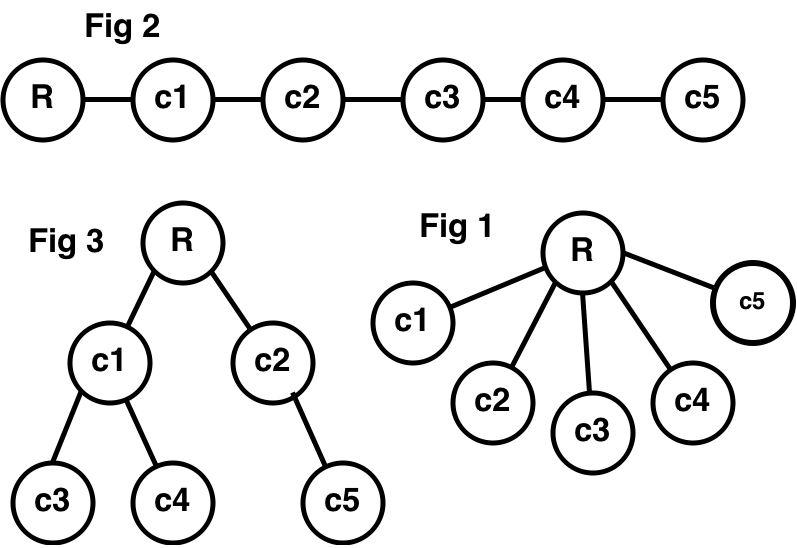
\includegraphics[width=120mm]{trees}
\caption{Different ways of organising distributed hash computations.}
\label{fig:trees}
\end{figure}

$R$ does the following work:
\begin{enumerate}
\item $R$ is padding the message to hash and divides the message into $B$ blocks. The frequency $f_{i}$ for each device $i$ and the total frequency $F$ for all devices are calculated. 
\item A balanced tree is created with all machines in the network as shown in \ref{fig:trees}. The order of the machines does not matter, but it seems reasonable to put the weakest machines at the bottom of the tree.
\item $R$ distributes $b$ random blocks to each device $i$ with frequency $f_{i}$, such that $b = \lceil \frac{B*f_{i}}{F} \rceil$.
\item $R$ sends the blocks, a reference to the parent, a boolean value indicating if the device is a leaf in the computation tree and a distributed hash function $P$ to the machine.
\item After $R$ has distributed the blocks, it waits for its two children to return the hashes $h_{1}$, $h_{2}$ and calculates the final hash by doing $h_{1} \oplus h_{2}$.
\end{enumerate}

The program $P$ looks like this:
\begin{verbatim}
ComputeHash(blocks, parent, is_leaf)
byte[] M = 0
foreach block in blocks {
    M = M <XOR> H(block)
}
if (!is_leaf) {
    wait for messages M_1 and M_2 from children
    send M <XOR> M_1 <XOR> M_2 to parent
}
send M to parent
\end{verbatim}

If the blocks are on a shared network resource, we must alter the program slightly. Instead of $R$ sending the blocks to hash, it sends the total frequency $F$ and a pointer to the first block to hash. Then $P$ would look like this:
\begin{verbatim}
ComputeHash(F, *first_block, parent, is_leaf)
byte[] M = 0
num_blocks = (frequency for this device / F) * sizeof(blocks)
for i = 0 to num_blocks {
    block = *(first_block + i)
    M = M <XOR> H(block)
}
if (!is_leaf) {
    wait for messages M_1 and M_2 from children
    send M <XOR> M_1 <XOR> M_2 to parent
}
send M to parent
\end{verbatim}
Nota bene: If the number of blocks is small, some machines might be left out of the computation. Also note that XOR is commutative so the order in which the blocks are XOR:ed together does not affect the final result, nor does the number of blocks each machines process, due to each block being hashed separately.

  \end{subproblem}
  \begin{subproblem}
    (3T) See above.
  \end{subproblem}
  \begin{subproblem}
    (5T) Since we have made the assumption that $H$ is collision resistant, we need to show that: Given a message $M = M_{1} || M_{2} \ldots || M_{B}$, hashing each block $M_{i}$ separately yields a collision resistant hash, i.e given that $H(M)$ is collision resistant $H(M_{1}) \oplus H(M_{2}) \ldots \oplus H(M_{B})$ is collision resistant.
    
    If we assume random oracle model, i.e there exists a "perfect" hash function then the XOR of two outputs from this hash function is collision resistant because the output will be completely random as well. 
    
    Suppose we have two messages $A$ and $B$ and we compute $H(A)$ and $H(B)$. The bits in these two hashes are random meaning:
    
    \begin{enumerate}
    \item No bit is biased (the probability of a bit being 1 is equal to the probability of a bit being 0)
    \item Each bit is independent from all the other bits.
    \end{enumerate} 
    An XOR operation preserves these two properties because:
    \begin{enumerate}
    \item For the four possible inputs 10, 01, 00, and 11, the probability of outputting a 0-bit is $\frac{1}{2}$ (11, 00) and the probability of outputting a 1-bit is $\frac{1}{2}$ (10, 01). Thus, the probability of a bit being 1 is the same in both $H(A), H(B)$ and $H(A) \oplus H(B)$.
    \item Each bit is calculated separately, and thus no output bit from the XOR operation depend on any other bit.
    \end{enumerate} 
    
    If the output from the XOR operation is random, it is no easier to find a collision from $H(A) \oplus H(B)$ than it is to find a collision for $H(A)$ and $H(B)$ respectively.
  \end{subproblem}
\end{problem}

\begin{problem}
  \begin{subproblem}
    (4T)
    In the paper they assume that the encryption algorithms are safe to use, in the sense that the best cryptographic attack during the lifetime of the data will be a brute-force attack where you will have to try all possible key combinations until the right key is found. Thus, the only thing that matters is how deep the pockets of your attacker is (more money means that yu can buy more processing power). The paper divides enemies into five categories: 
    \begin{enumerate}
    \item A hacker with a PC or maybe a special-built.
    \item Small organisation with FPGA-hardware and about 100 thousand SEK.
    \item Medium organsiation with special-built ASIC-hardware and about 3 million SEK.
    \item Big organsation with 100 million and FPGA or ASIC hardware.
    \item Intelligence agency with 3 billion SEK and ASIC-hardware.
    \end{enumerate}
    The formula for determining the key size is to choose an $n$-bit key such that $\frac{2^n}{P}$ is larger than the lifetime of the data. $P$ is the processing power of the enemy, say number of keys which can be tested on one day. The value of $P$ is based on a paper by Blaze et. al. which suggests that a hacker with a FPGA can test about $2^{40}$ keys per day, a small organisation can test $2^{47}$ keys per day, a medium organisation can test $2^{50}$ keys per day, a large organisation can test $2^{63}$ keys per day and an intelligence agency up to $2^{70}$ keys per day, yielding a minimum recommended keysize of e.g 75 bits for an intelligence agency.
    
    In the paper they discuss the possibility of a distributed attack, i.e using a botnet to test keys, concluding that they need to add another category of "a distributed attacker", suggesting another 20 bits is added to this category.
    The paper also discusses the usage of GPU (instead of CPU) to speed up the search for keys. They suggest that another five bits is added.
    Motivated by the development of faster machines, FPGA:s and ASIC:s, they draw the conclusion that Moore's law is needed to be taken into account by adding another 8 bits to all categories (since the work by Blaze et. al. is from 1996).
    
    Asymmetric key size (RSA) is determined based on the GNFS-algorithm for factoring large numbers (quantum computers are assumed not be a reality in near future), giving the following rule of determining equivalent symmetric key size for an RSA modulus with $x$ bits:
    \[
    f(x)=\frac{64}{9}^{\frac{1}{3}}log_{2}(e)(x\ln(2))^{\frac{1}{3}}(\ln(x\ln 2 ))^{\frac{2}{3}}-14
    \]
    The effective keysize a $n$-bit DLOG or elliptic curve key is given by $\frac{n}{2}$.
    
    \begin{figure}
    \centering
    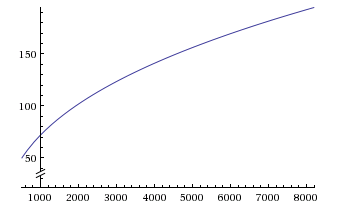
\includegraphics[width=80mm]{gfns}
    \caption{Asymmetric key size and corresponding symmetric key size.}
    \label{fig:gfns}
    \end{figure}
    
  \end{subproblem}
  \begin{subproblem}
    (2T) For example, we can extend table 7.2 with a row of 512 bits of security as follows: Number of bits $x$ in the RSA-modulus would be $f^{-1}(512)$, i.e the root to the equation $\frac{64}{9}^{\frac{1}{3}}log_{2}(e)(x*\ln(2))^{\frac{1}{3}}(\ln(x*\ln 2 ))^{\frac{2}{3}}-526 \rightarrow x \approx 82030$ bits. Due to half the size-principle, the corresponding EC-key must have $2*512=1024$ bits.
    
    Table 7.3 is extended by calculating $f(x)$. Example: Suppose we want to extend table 7.3 with an RSA/DLOG key of 4096 bits. The security column (column 2) would then be $f(4096) = \frac{64}{9}^{\frac{1}{3}}log_{2}(e)(4096*\ln(2))^{\frac{1}{3}}(\ln(4096*\ln 2 ))^{\frac{2}{3}}-14 \approx 142$ bits.
  \end{subproblem}
  \begin{subproblem}
    (1T) I believe that in the future, discrete logarithm in elliptic curves will be more widespread than cryptography based on integer factorisation, due to the fact that DLOG in elliptic curves allows for smaller key sizes. Also, crypto based on integer factorisation will not be secure if quantum computers become a reality due to Shor's algorithm.
  \end{subproblem}
\end{problem}

\begin{problem}
  \begin{subproblem}
    (1T)
    \[
    y^c\alpha = g^d \textit{ mod N }
    \]
    \[
    y^c(g^r \textit{ mod N}) = g^d \textit{ mod N}
    \]
    \[
    y^c(g^r \textit{ mod N}) = g^{xc+r} \textit{ mod N}
    \]
    \[
    (g^x \textit{ mod N})^c(g^r \textit{ mod N}) = g^{xc+r} \textit{ mod N}
    \]
    \[
    (g^x)^c g^r \textit{ mod N} = g^{xc+r} \textit{ mod N} 
    \]
    \[
    g^{xc}g^r = g^{xc+r}
    \]
    \[
    g^{xc}g^r=g^{xc}g^r
    \]
  \end{subproblem}
  \begin{subproblem}
    (3T) NOT SOLVED % We leave this place holder here for improved readability.
  \end{subproblem}
  \begin{subproblem}
    (2T) NOT SOLVED % We leave this place holder here for improved readability.
  \end{subproblem}
\end{problem}


\begin{problem}
  \begin{subproblem}
    (2T) Lamport signatures uses some kind of hash function $H$, say SHA-256 and a PRNG.
    
    The private key is constructed by generating 256 pairs of random numbers $(x_{1}$, $y_{1})$, $(x_{2}, y_{2})$...
    $ (x_{256}, y_{256})$ using the PRNG. The public key consists of the hashes $(H(x_{1}), H(H(y_{1}))$, $(H(x_{2})$, $H(y_{2})) \ldots (H(x_{256})$, $H(y_{256}))$. The private key cannot be derived from the public key because $H$ is pre-image resistant. 
    A signature is created as follows: 
    \begin{itemize}
    \item The message $M$ is hashed. The hash is $H(M) = b_{1},b_{2}\ldots b_{256}$.
    \item For each bit $b_{i}$ in the hash, the signer selects the $b_{i}$:th random number from the $i$:th pair in the secret key. This will be the signature for the message (consisting of 256 random numbers).
    \end{itemize} 
    A signature is verified like this:
    \begin{enumerate}
    \item The verifier hashes the message $H(M) = b_{1},b_{2}\ldots b_{256}$ and each of the 256 random numbers in the signature.
    \item For each bit $b_{i}$ in the hash, the verifier compares the $i$:th hash in the signature with the $b_{i}$:th hash in the public key. If all 256 hashes match, the signature is correct. 
    \end{enumerate}
  \end{subproblem}
  \begin{subproblem}
    (1T) Since the signature reveals half of the private key, it cannot be reused. Given that an attacker gets hold of a signature (which is public), she would just have to guess the pre-image for half the hashes to restore the private key.
  \end{subproblem}
\end{problem}

\end{document}
